\documentclass[a4paper, twoside, 10pt]{report}

\newcommand{\finalcommand}{}

% !TEX root = BachelorBookletMain.tex

\def\hiddencol{rgb:black,0.5;white,10;violet,1.5}
\def\inputcol{rgb:black,0.5;white,10;green,1}
\def\outputcol{rgb:black,0.5;white,10;red,1.5}

\newcommand{\neuron}[5]{
	\node [circle, fill={#5},draw=black,inner sep=2mm,minimum size=1.2cm](#3) at (#1,#2) {#4};
}

\newcommand{\multilayerNetworkGraph}[1][b]{
	\begin{figure}[#1]
	\begin{center}
	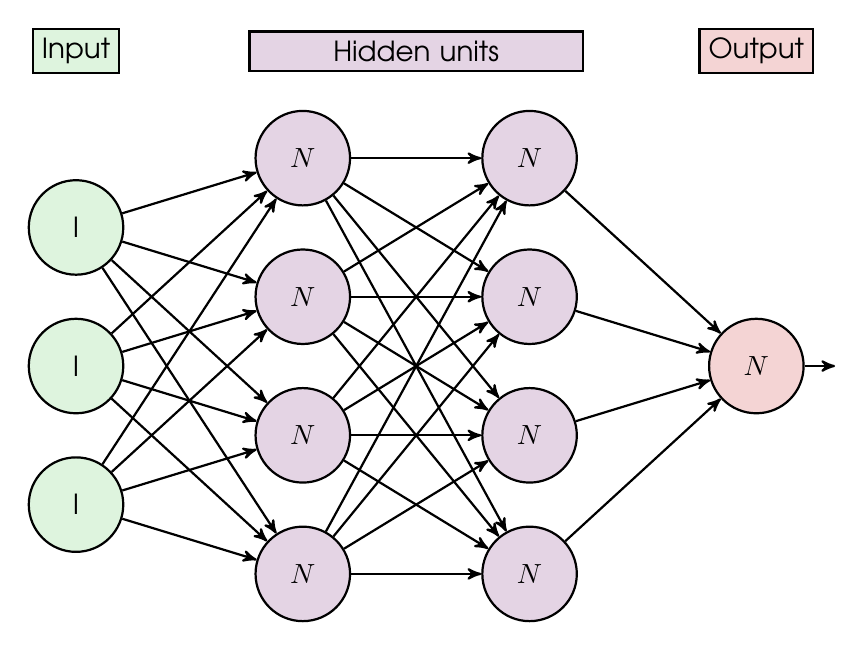
\begin{tikzpicture}[thick,>=stealth']
		\def\csunit{cm}
		\def\circleSize{0.8}
		\def\layerdist{3.6}

		\def\mcOne{2}
		\foreach\n in {0,...,\mcOne}{
		 \FPeval{\ypos}{(\n - (\mcOne * 0.5)) * 2.2}
		 \neuron{0 * \layerdist}{\ypos * \circleSize\csunit}{A\n}{I}{\inputcol}
		}
		\def\mcTwo{3}
		\foreach\n in {0,...,\mcTwo}{
		 \FPeval{\ypos}{(\n - (\mcTwo * 0.5)) * 2.2}
		 \neuron{\circleSize\csunit*\layerdist}{\ypos * \circleSize\csunit}{B\n}{$N$}{\hiddencol}
		 \foreach\m in {0,...,\mcOne}
			\draw[->, to path={-> (\tikztotarget)}] (A\m) edge (B\n);
		}
		\def\mcThree{3}
		\foreach\n in {0,...,\mcThree}{
		 \FPeval{\ypos}{(\n - (\mcThree * 0.5)) * 2.2}
		 \neuron{\circleSize\csunit*\layerdist*2}{\ypos * \circleSize\csunit}{C\n}{$N$}{\hiddencol}
		 \foreach\m in {0,...,\mcTwo}
			\draw[->, to path={-> (\tikztotarget)}] (B\m) edge (C\n);
		}
		\def\mcFour{0}
		\foreach\n in {0,...,\mcFour}{
		\FPeval{\ypos}{(\n - (\mcFour * 0.5)) * 2.2}
		 \neuron{\circleSize\csunit*\layerdist*3}{\ypos * \circleSize\csunit}{D\n}{$N$}{\outputcol}
		 \foreach\m in {0,...,\mcThree}
			\draw[->, to path={-> (\tikztotarget)}] (C\m) edge (D\n);
		}
		\FPeval{\xpos}{\circleSize*\layerdist*3 + 1}
		\draw[->, to path={-> (\tikztotarget)}] (D0) edge (\xpos\csunit,0);

		\def\colD{rgb:black,1;white,10;violet,1}
		\FPeval{\ypos}{\mcThree + 1}

		\node[fill={\inputcol},draw,align=left] at (\circleSize\csunit*\layerdist * 0, \ypos) {Input};
		\node[fill={\hiddencol},draw,text width=4cm, align=center] at (\circleSize\csunit*\layerdist *1.5, \ypos) {Hidden units};
		\node[fill={\outputcol},draw,align=left] at (\circleSize\csunit*\layerdist *3, \ypos) {Output};
	\end{tikzpicture}

	\caption{Multilayer neural network structure}
	\figsource{Own graphic}
	\label{multilayerNetworkGraph}

	\end{center}
	\end{figure}
}

\newcommand{\neuronGraph}[2]{
	\begin{figure}[#1]
	\begin{center}
	\begin{tikzpicture}[thick,>=stealth']

			\neuron{0}{0}{N}{#2}{\hiddencol}
			\node (I1) at (-5,3){$\boldsymbol{x}_1$};
			\node (I2) at (-5,0){$\boldsymbol{x}_2$};
			\node (I3) at (-5,-3){$\boldsymbol{x}_3$};
			\path[->]
				(I1) edge [left] node [pos=0.5, sloped, above] {$\boldsymbol{w}_1$} (N)
				(I2) edge node [pos=0.5, sloped, above] {$\boldsymbol{w}_2$} (N)
				(I3) edge node [pos=0.5, sloped, above] {$\boldsymbol{w}_3$} (N)
				(N) edge (5,0);

	\end{tikzpicture}
	\end{center}

	{
	\caption{Graphical representation of a neuron with 3 inputs}
	\figsource{Own graphic}
	\label{neuronGraph}
	}

	\end{figure}
}

\newcommand{\GQNArchitectureGraph}{
\begin{figure}
\centering
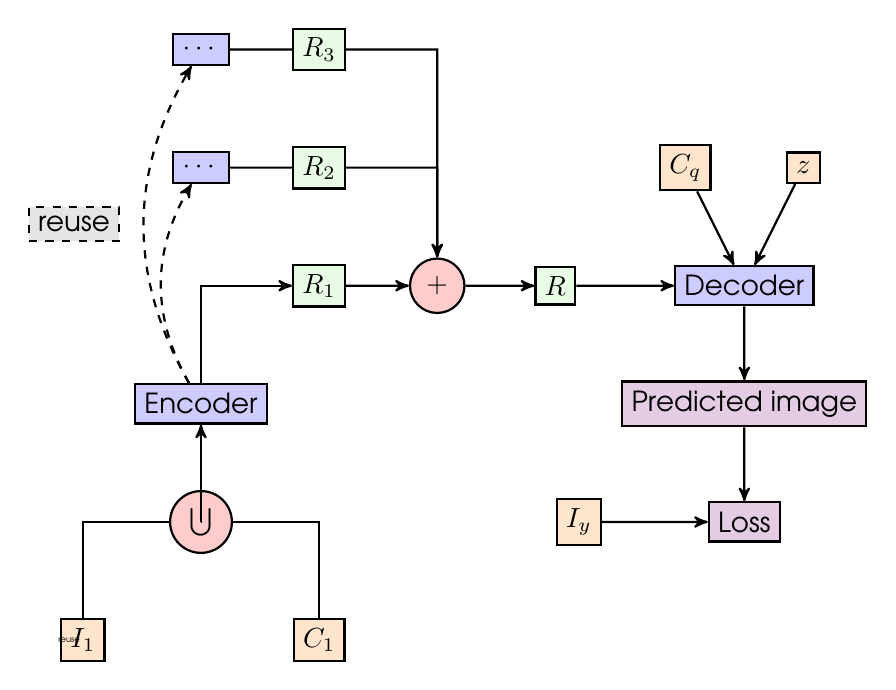
\begin{tikzpicture}[->, thick, >=stealth', scale=0.3]

	\def\cR{red!10!green!10!white}
	\def\cNet{blue!20!white}
	\def\cOp{red!20!white}
	\def\cVar{orange!20!white}
	\def\cOut{violet!20!white}

	\path
		(0,0) node[draw, fill=\cVar] (oImage) {$I_1$}
		++(5,5) node[circle, draw, fill=\cOp] (append) {$\bigcup$}
		+(5,-5) node[draw, fill=\cVar] (coordinate) {$C_1$}
		++(0,5) node[draw, fill=\cNet] (encoder) {Encoder}
		++(5,5) node [draw, fill=\cR] (r_1) {$R_1$}
		++(0,5) node [draw, fill=\cR] (r_2) {$R_2$}
		++(0,5) node [draw, fill=\cR] (r_3) {$R_3$}
		(r_1) ++(5,0) node [circle, draw, fill=\cOp] (add) {$\bm+$}
		++(5,0) node [draw, fill=\cR] (r) {$R$}
		++(8,0) node [draw, fill=\cNet] (decoder) {Decoder}
		+(2.5, 5) node [draw, fill=\cVar] (z) {$z$}
		+(-2.5, 5) node [draw, fill=\cVar] (querryCoord) {$C_q$}
		++(0, -5) node [draw, fill=\cOut] (output) {Predicted image}
		++(0, -5) node [draw, fill=\cOut] (loss) {Loss}
		+(-7, 0) node [draw, fill=\cVar] (label) {$I_y$}
		;

	\draw (coordinate) |- (append)
						(oImage) |- (append) -| (encoder);
	\draw (encoder) |- (r_1);
	\foreach \n in {r_2, r_3}
		\draw (\n) ++(-5,0) node[draw, fill=\cNet] (dot_\n) {$\cdots$} -- (\n)
					(\n) -| (add);
	\draw (encoder) edge[bend left, dashed] (dot_r_2)
				(encoder) edge[bend left, dashed] node[left=3mm, draw, fill=black!10!white] {reuse} (dot_r_3);
	\draw (encoder) node[pos=0.5, sloped, left] {reuse} (dot_r_3);
	\draw (r_1) edge (add)
				(add) edge (r)
				(r) edge (decoder)
				(decoder) edge (output)
				(output) edge (loss)
	 			(querryCoord) edge (decoder)
	 			(z) edge (decoder)
				(label) edge (loss)
				;

\end{tikzpicture}

\caption{GQN architecture}
\figsource{own graphic}
\label{GQNArchitectureGraph}

\end{figure}
}


\usepackage{fancyhdr}
\usepackage{color}
\usepackage{afterpage}
\usepackage{graphicx}
\usepackage{amsmath, amsfonts, amssymb}
\usepackage[ddmmyyyy]{datetime}
\renewcommand{\dateseparator}{.}
\usepackage{setspace}
\usepackage{titlesec}
\usepackage{tikz}
\usetikzlibrary{calc,arrows,shapes,snakes,automata,backgrounds,petri}
\usepackage[margin=5cm]{geometry}
\usepackage{avant}
\usepackage{makecell}
\usepackage[english]{babel}
\usepackage{wrapfig}
\usepackage{ragged2e}
\usepackage{pgfplots}
\pgfplotsset{compat=1.16}
\usepackage{pgffor}
\usepackage{fp}

\setstretch{1.3}
\setlength{\parskip}{1em}

\titleformat{\chapter}
	{\normalfont\huge\bfseries}{\thechapter}{1em}{}
\titlespacing*{\chapter}{0pt}{3.5ex plus 1ex minus .2ex}{2.3ex plus .2ex}

\AtEndDocument{\cleardoublepage}

\title{Bachelor thesis booklet}
\author{Johannes C. Mayer}
\date{\today}

\newcommand\blankpage{\null\thispagestyle{empty}\addtocounter{page}{0}\newpage}
\renewcommand{\familydefault}{\sfdefault}

\pagestyle{fancyplain}
\fancyfoot{}
\fancyfoot[le,ro]{{\small \thepage} \\[4mm] }

\usepackage[list=true]{subcaption}
\usepackage{tocloft}
\setcounter{lofdepth}{2}
\makeatletter
\newcommand{\figsourcefont}{\footnotesize}
\newcommand{\figsource}[1]{%
  \addtocontents{lof}{%
    {\leftskip\cftfigindent
     \advance\leftskip\cftfignumwidth
     \rightskip\@tocrmarg
     \figsourcefont#1\protect\par}%
  }%
 }
\makeatother

% HOW TO USE ^^^^
%\begin{figure}[hbt]
%\centering
% {\caption{Caption}
%    \figsource{Source}}
%       \subcaptionbox{Caption1}
%{
\includegraphics[width=0.4\textwidth]{images/FrontCover.png}}
%       \figsource{Source1}
%\subcaptionbox{Caption2}
%{ 
\includegraphics[width=0.4\textwidth]{images/FrontCover.png}}
%        \figsource{Source2}
%\end{figure}

\begin{document}

\begin{titlepage}
\begin{tikzpicture}[remember picture,overlay]
	\node[inner sep=0pt] (background) at (current page.center) {
\includegraphics[width=\paperwidth]{images/FrontCover.png}};
	\draw ($(current page.south)+(0,5)$) node [fill=black,fill opacity=0.6,text opacity=1,inner sep=1cm]{\color{white}\Huge\centering\bfseries\sffamily\parbox[c][][t]{0.7\paperwidth}
	{Shrouded Mirror\\[0pt]
	{\Large Neural Network Based Rendering \\[-6mm] in Interactive Environments}\\[0cm]
	{\large Johannes C. Mayer}}};
\end{tikzpicture}
\end{titlepage}


\blankpage
eeeeeeeee

\pagenumbering{Roman}
\begin{flushleft}
\begin{spacing}{1.5}
{\large
Bachelor thesis booklet in the studies of GAME DESIGN \\
%\vspace*{\fill}
The work constitutes a technical design work piece \\
\vspace*{\fill}
{\Huge Shrouded Mirror} \\
{\Large Neural Network Based Rendering \\ in Interactive Environments \\}
\vspace*{\fill}
\textit{Submitted by} \\
Johannes C. Mayer, 553087 \\
on \today \\
\vspace*{1cm}
\textit{First Examiner:} Prof. Thomas Bremer \\
\textit{Second Examiner:} Prof. Susanne Brandhorst \\
\vspace*{1cm}
Hochschule f\"ur Technik und Wirtschaft Berlin \\
Fachbereich Gestaltung und Kultur \\
}
\end{spacing}
\end{flushleft}

% !TEX root = BachelorBookletMain.tex

\chapter*{Expos\'e}
In my bachelor thesis I want to evaluate how neural networks can be used in an interactive context to visualize an environments state. For this the project is structured into three phases. First create a simple implementation of the algorithms required, then explore possible applications, third develop the most promising application further.

Neural networks have the ability to learn an abstract representations of the data they are being trained on. This representation can then be used to generate new output. In this work a network is used that is trained on data pairs that consist of an Image and the corresponding coordinates where the image was taken.  The network can now, given a set of scene coordinates, render an image that approximates what a camera would render when placed at the provided coordinates. This means that this technique can be used to create a second visual representation of an environment inside a game engine.

Interesting possibilities open when integrating this network into an interactive environment. One example would be, that the player only sees the output of the network while the underlying “real” state of the environment is hidden from him.

%\subsubsection{Workflow}
%The Project will be split up into three phases. Each phase will result in a prototype, that the following phase builds on.
%
%\paragraph{I.  Implementation}
%Determine which library to use. PyTorch, Chainer, Keras, Tensorflow are possible candidates. The first two might be prefered due to their ability to define computation graphs dynamically which would possibly allow the output size of the GQN to scale with screen size. With the selected library, a GQN is implemented into the target environment (most likely Unity).ii
%
%\paragraph{II. Exploration}
%The implementation of the GQN will now be investigated in regards to its manipulability and  constraintsivenes. The following questions will be answered:
%
%Is it viable to inject additional parameters into the model, to enable more interesting behaviour?
%What are the time constraints of applying a GQN into an interactive real time environment (training time, rendering time, updating worldmodel)?
%
%Can a normal in game camera be overlayed with the output of the GQN?
%Can objects be made to switch contexts of being displayed via GQN or camera dynamically?
%Which interesting ways of interaction between player and the way the GQN behaves can be created, given other constraints?
%
%\paragraph{III. Simple Application}
%With the Gathered data on the limitations and possibilities a simple prototype application is conceptualized and developed. It demonstrates one or multiple scenarios in which the GQN can be applied to create or enhance an interactive environment.
%
%\subsubsection{Work piece}
%The following items will be produced during the Project:
%\begin{itemize}
%\item{Writing}
%\item{Discussion of the Results form prototype II}
%\item{Reflection on the project}
%\item{Executable and source of prototype III}
%\item{1 - 5 minutes video material, captured from interactions with prototype III}
%\end{itemize}
\clearpage


\tableofcontents
\clearpage

\pagenumbering{arabic}


% !TEX root = BachelorBookletMain.tex

\chapter{Introduction}
Shrouded mirror is an experimental experience, where the player sees the world through the eyes of a neural network. The player moves through an environment, collects beacons and avoids enemies. Each type of entity emits a unique audio signal, creating a distinctive soundscape.
\begin{figure}[hbt]
\centering
    
\includegraphics[width=0.4\textwidth]{images/FrontCover.png}
    \caption{Test caption of img}
    \figsource{Own graphic}
\end{figure}

\section{Motivation}
Using the representation of an environment a neural network has learned, to present the state of an environment to the player is still an nearly unexplored avenue.
In this work I explore how neural networks can be used to create a unique interactive experiences, by using the output the neural representation of the network produces as the main information stream presented to the player.

\section{Scope}
what has been done, what pieces constitute the work?
During the bachelor thesis the following things where developed:

\begin{itemize}
\item{Data generation environment}
\item{Data processing pipeline}
\item{Scene rendering neural network model and training pipeline}
\item{System to send network output in Unity}
\item{Merging of network output with unity rendered objects}
\item{Several exploratory prototypes}
\item{One extended Prototype (Maze game)}
\end{itemize}

% !TEX root = BachelorBookletMain.tex

\newcommand{\neuronSum}[1][n]{
	\sigma\Bigg(\sum_{i=1}^{#1}{\Big(w_i x_i\Big)} + b\Bigg)
}

\chapter{Background}
\section{Neural networks}
To give a better intuition for how neural networks work and how they are used in this project, a brief overview follows describing the components necessary to build a simple neural network.

In brief a neural network is computational structure made up of multiple units called neurons that can adapt their output based on data.


\subsection{Neuron}
A simple neuron can be defined as:

\begin{equation}
\begin{split}
	N_{\bm w, b}(\bm{x}) & = \neuronSum[n] \\
 	& = \sigma (\bm{w} \cdot \bm{x} + b)
\end{split}
\end{equation}

Where $\bm{x} \in \mathbb{R}^n$ is a vector containing all inputs, $ \bm{w} \in \mathbb{R}^n$ a vector containing the neurons weights, $b \in \mathbb{R}$ is the bias, $n \in \mathbb{Z}$ is the number of inputs and $\sigma$ is a nonlinear function refereed to as the activation function of the neuron. $\sigma$ is often set to be the rectified linear unit $ReLU(x) = \max(0, x)$.

Intuitively a neuron performs a weighted sum over its inputs adds a bias and applies an activation function to the result to calculate the final output. The bias can be thought of as a threshold, determining---if $\sigma = ReLU$---how high the sum of inputs has to be, before the output becomes non 0. Figure \ref{neuronGraph} shows, how we can think of as a neuron having connections.

\neuronGraph{p}{$\displaystyle{\neuronSum[3]}$}


\subsection{Multilayer network}
As seen in figure \ref{multilayerNetworkGraph} a neural network work can be formed out if neurons, by first organizing multiple neurons into a layers and then connecting multiple layers together. To get a dense network, each neuron in a layer gets as inputs the outputs of all the neurons in the previous layer. The first layer is used to provide input to the network. We simply set the output values of the neurons to what we like to have as input to the network. To get the output of the network, we read of what values the neurons in the final layer have after the network has been evaluated. The layers between the first and last layer are called hidden layers. This is because it is normally not necessary to inspect directly what values these neurons have.

\multilayerNetworkGraph[p]

Normally in an implementations of a densely connected neural network the computer performs multiple matrix operations to compute the output to be more efficient. Equation \ref{networkMatrixMul} shows how to compute the values for the first hidden layer of the network in figure \ref{multilayerNetworkGraph} this way. The $\sigma$ is applied to each element of the vector.

\begin{equation}
	Hidden_1(\bm{x}) = \sigma\Bigg{(}
	\directlua{
		print_matrix('w', 4, 3)
		print_matrix('x', 3)
		tex.print('+')
		print_matrix('b', 4)
	}
	\Bigg{)}
	\label{networkMatrixMul}
\end{equation}


\subsection{Training}
Before we start training we need to set our weights and biases to some start values.
The bias is usually initialized to 0 and the weights can be initialized to small random values if the network is small. More complicated initialization strategies are needed for the weights if we are dealing with a big network (\cite{Glorot2010-kn,Ioffe2015-eh}).

Normally we are interested in finding specific weight vectors and biases for neurons that make the network perform some specific task like image classification, given some data.

We might want to know if an image pictures a orange or an apple. We can use a network with one output neuron, where that neurons value should be one if we feed in a picture of an orange and zero if we feed in a picture of an apple. if we now feed in a picture, the network gives back some arbitrary numerical value that will only by chance predict the correct fruit. This is because the network is not trained yet.

To train the network we first need to define a loss function. This function returns a numerical value, that represents how bad the network is. For images we may use the means square error function as shown in equation \ref{MSE}. There $x$ is the output of the network and $y$ is the output that we want.

\begin{equation}
	MSE(\bm{x}, \bm{y}) = \frac{1}{n}\sum_{i=1}^{n}{(\bm{x}_i - \bm{y}_i)^2}
	\label{MSE}
\end{equation}

To train the network we need a dataset, that in this case an image, paired with the number one if the image depicts an orange and the number zero if the image depicts an apple.

Now if we feed in an image into the network we can measure how bad the network is using the loss function. To improve the output of the network we train it by updating our weight and bias values corresponding to the negative gradient of the loss function with respect to the weights and biases using calculus.


\section{Differential calculus}
Differential Calculus is an area of mathematics, that studies how a functions output changes with regard to tiny nudges to its inputs.


\subsection{Univariate}
The derivative says how much the output of a function increases, at a specific point. It is defined as:

\begin{equation}
	\frac{df(x)}{dx} = \lim_{dx \to 0}\frac{f(x + dx) - f(x)}{dx}
\end{equation}

Intuitively this can be interpreted as the amount the output of the function changes when we increase the parameter to function by some tiny amount divided by how tiny that amount was. The $\lim_{dx \to 0}$ means, that we don't use a specific value for $dx$ but take the value the equation approaches when $dx$ approaches $0$, without $dx$ ever becoming $0$.

This means that the derivative can be used to find out how a function changes locally. If the derivative is positive and we increase the input to the function at the point the derivative was evaluated the output increases in size proportional to the magnitude of the derivative. The same logic applies when the derivative is negative.


\subsection{Multivariate}
The same can be applied to functions with multiple parameters:

\begin{equation}
\begin{split}
	\frac{\partial f(x_1, x_2)}{\partial x_1} = \lim_{\partial x_1 \to 0}\frac{f(x_1 + \partial x_1, x_2) - f(x_1, x_2)}{\partial x_1} \\
	\frac{\partial f(x_1, x_2)}{\partial x_2} = \lim_{\partial x_2 \to 0}\frac{f(x_1, x_2 + \partial x_2) - f(x_1, x_2)}{\partial x_2}
\end{split}
\end{equation}

Here each equation defines as how much the output of the function changes locally when the corresponding input parameter to the function varies.
The gradient of $f(x_1, x_2)$ is defined as:

\begin{equation}
\nabla f(x_1, x_2) =
	\begin{bmatrix}
	\frac{\partial f(x_1, x_2)}{\partial x_1} \\[2mm]
	\frac{\partial f(x_1, x_2)}{\partial x_2}
	\end{bmatrix}
\end{equation}

This means the gradient contains all the information, of how a function varies with respect to its parameters.

Calculating the gradient of the loss, gives us the information of how we should adjust our weights and biases to improve the loss i.e. the output of the network. Normally we scale the gradient by some learning rate $\eta \in \mathbb{R}$.


% \subsection{Backpropagation}
% In practice neural networks are constructed as computation graphs. This means a the computations are defined by how edges connect to nodes, where the nodes correspond to operations to be performed.
% Define computation graph, to enable reverse mode auto diff.


\section{GQN Network}\label{BackgroundGQN}
\subsection{Definition}
A Generative Query Network (\cite{gqn}) is a type of neural network architecture, that can learn how to render an image from a given viewpoint in an environment\footnote{Environment here refers to a scene that contains certain objects---like walls and spheres---arrangement in a certain way.} not seen during training, given only a handful of images of the environment. The closer the unseen environment is to environments seen during training---in terms of objects and their properties---the better the network is generally expected to perform on the unseen environment. To some extend the network is able to correctly render unseen objects as shown by \cite{gqn}.

The network architecture is shown in figure \ref{GQNArchitectureGraph}, where $I_i$ denotes an image of an environment and $C_i$ the position and rotation where the image was taken. The $\bigcup$ here means concatenation. $R_i$ is an encoded representation of the environment as a tensor. These tensors are summed up element wise. $C_q$ is the coordinate from which the network should render an Image, $z$ is a vector of latent variables and $I_y$ is the ground truth image of what a render form $C_q$ looks like. The encoder and decoder are both neural networks.

To train the network we feed many image-coordinate pairs, from different environments, compute the gradient of the loss and update the network parameters accordingly. All $(I_i, C_i)$ and $(I_y, C_q)$ have to be drawn from the same environment in one evaluation of the network. If there are multiple $(I_i, C_i)$ input pairs, the same encoder network is used to encode each of them.

\GQNArchitectureGraph


\subsection{Usage}
This work uses a simplified implementation of the Generative Query Network.

In this work a network the architecture of GQN differs from the implementation used in the original paper. Here I use simple dense models for encoder and decoder that don't use random latent variables. This circumvents the necessity of having to use the evidence lower bound as an optimization target.

This however prevents the network from taking into account the inputs given during inference to the same extent as in the original experiments described in the paper. The only meaningful considerations of the inputs of the network were found to be the coloring of the sky, floor and walls (when the latter view have the same color). In the original implementation the network can correctly infer more properties like object position, rotation and texture.

Because interesting use cases where found, that do not depend on this property of the GQN network no more effort was put into recreating the ability of the network to model different scenes.

% !TEX root = BachelorBookletMain.tex

\chapter{Workflow}
In this project I fallowed an iterative prototype workflow creating a prototype to evaluate a specific ideas. As for implementing different systems needed for the prototype I followed the workflow of researching a single component\footnote{such as the Kears functional API, UDP sockets, etc.} and implementing it, before beginning further researching efforts.

What fallows is a description of the prototypes developed over the course of the project. The main prototype "maze game" was the main focus of the project after the direction of the project was defined using the results from previous prototypes as guidance. It is described in detail in \cref{MazeGameSystems}.


\subsection{Functional}
The first prototype was developed with the intension of establishing the core systems. The entire data generation- and preprocessing pipeline and the neural network model where implemented and evaluated. A small level with checkerboard textures, seen in \cref{Functional}, and variable sky and wall colors between environments was created to evaluate the systems. \todo{make a distinction between environment and level everywhere in the document, where environment is a variation of a level}

\begin{figure}[p]
  \centering
  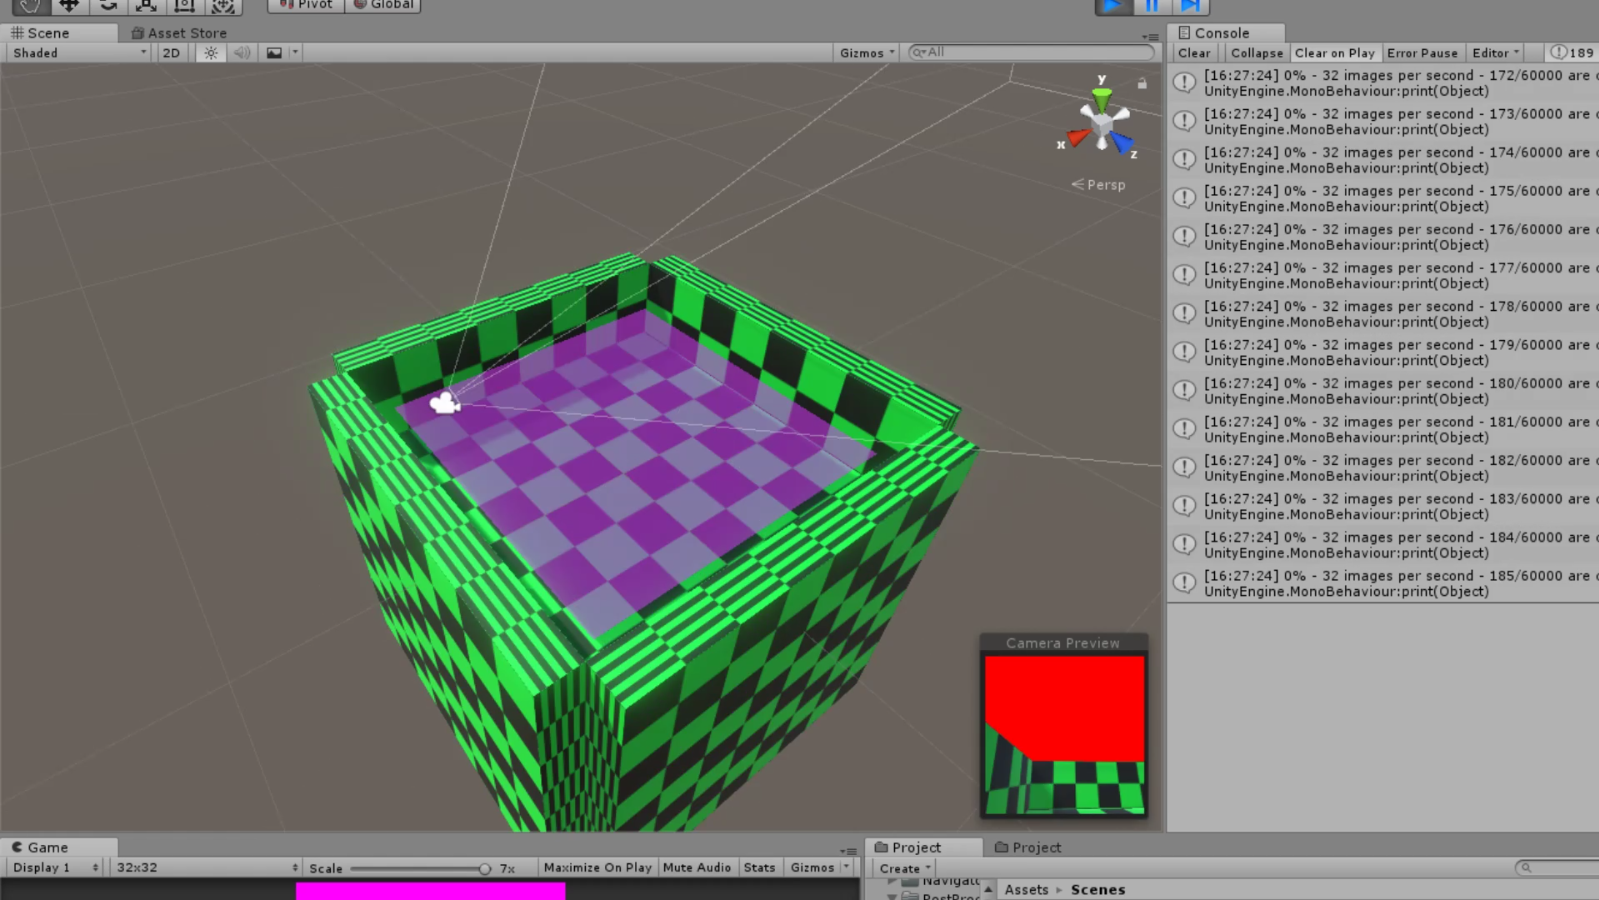
\includegraphics[width=\imgWidth]{images/workflow/Functional1.png} \\[\picVdist]
  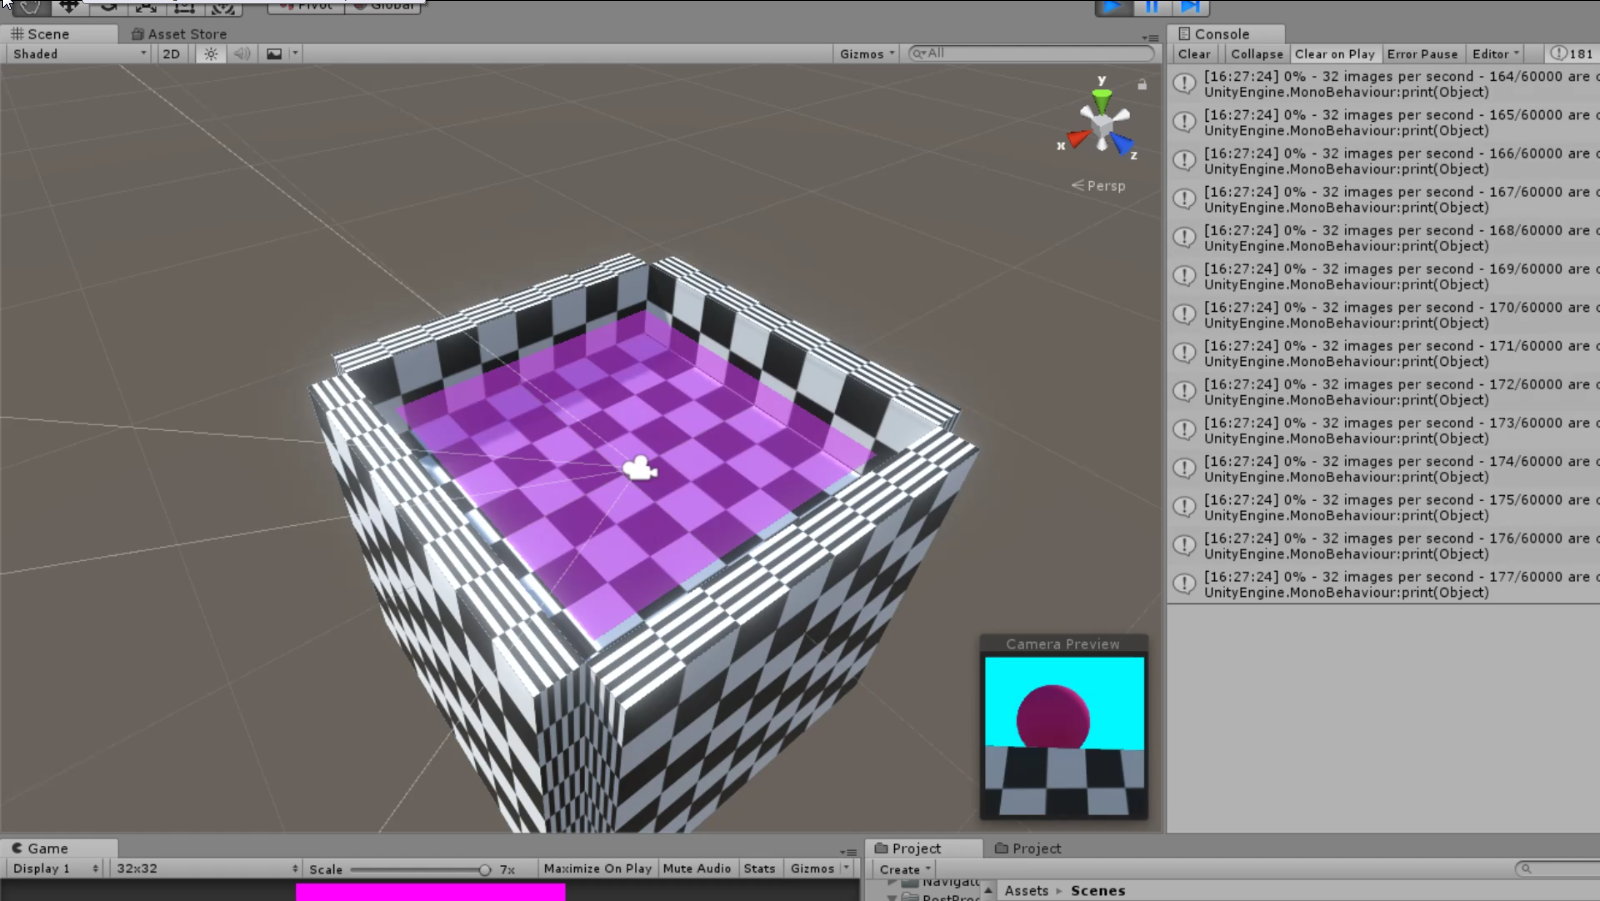
\includegraphics[width=\imgWidth]{images/workflow/Functional2.png}
  \caption{The environment of the functional prototype}
  \label{Funcional}
\end{figure}


\subsection{Top down}
This prototype was used to evaluate the suitability of the network for a top town game. In this prototype the player is supposed to go from one colored platform to another while avoiding running into red walls. The challenge should be created by only training the network on data captured when the camera points at one of the colored platforms. Training the network on this data resulted only in making the network output blurry, when the player was not positioned on a platform (see \cref{WalkOffPlatform}).

\begin{figure}[p]
  \centering
  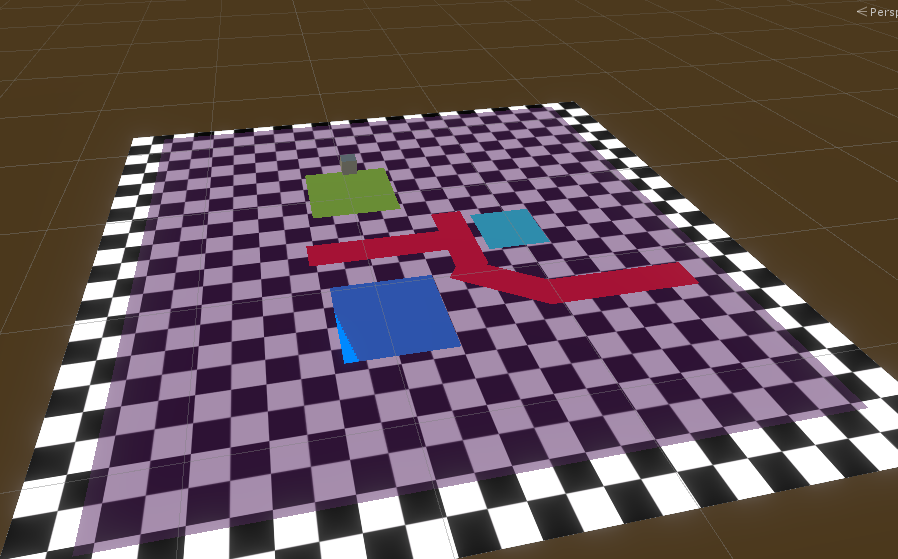
\includegraphics[width=\imgWidth]{images/workflow/TopDownLevel.png}
  \caption{Top down level as seen in the editor}
  \label{TopDownUnity}
\end{figure}

\begin{figure}[p]
  \centering
  
\includegraphics[width=\imgWidth]{images/workflow/TopDownOn.png} \\[\picVdist]
  
\includegraphics[width=\imgWidth]{images/workflow/TopDownOff.png}
  \caption{The network output gets blurry when the player walks off a platform.}
  \label{WalkOffPlatform}
\end{figure}


\subsection{Walking sim}
Here the idea was to use the neural network to present the environment to the player through the neural network to create an interesting visual appearance. It also was experimented with having certain objects only be visible if the player is a certain position in the environment (see \cref{WalkingSim}). This idea was further explored in the next prototype.

\begin{figure}[p]
  \centering
  
\includegraphics[width=\imgWidth]{images/workflow/WalkingSimNothing.png} \\[\picVdist]
  \includegraphics[width=\imgWidth]{images/workflow/WalkingSimClound.png}
  \caption{Objects can only be seen, when the player stands at certain locations}
  \label{WalkingSim}
\end{figure}


\subsection{Object morphing}
This prototype has a level that is divided into four differently colored platforms that are surrounded by tall pillars. The pillars and the coloring of the platforms help the player to orient himself. In the center four different objects are placed. Each of the object is linked with a different marker group as described in \cref{DataGeneration}. There is maker placed for each platform. This means that if an observation is taken from a specific platform only one object is displayed in the center. When the player crosses from one platform to another the center object is morphed from one object to another in an interpolated way. This is because if a network has a limited amount of parameters it can not model an instantaneous change in "pixel space".

\dl{cimg('picture without object')}
\dl{cimg('img of the morphing center object')}

\dl{cimg('img of the morphing center object')}

\dl{cimg('img of unity scene')}

% !TEX root = BachelorBookletMain.tex

\chapter{Systems}
\section{Model}
Model in python

\subsection{Network} \label{Network}


\subsection{Saving and loading}
\section{Data Preprocessing}
\section{Inter process communication}
UDP sending of player position to python

Motion JPEG over UDP socket

\section{Rendering}
In Unity the stream is decoded and rendered using custom Cg shaders. These shaders merges the network output stream with objects in the environment that are tagged to be visible in the combined render.

Cull objects if hidden from camera pos in unity environment

\section{Player interaction}
\paragraph{Laser}
player can shoot laser and destroy enemies

\paragraph{Smoke balls}
player can throw smoke balls which reveal invisible enemies and reveale the where the physical walls are in the smoke

% !TEX root = BachelorBookletMain.tex

\chapter{Further work}
In this section possible further applications based on the found data is discussed.

\section{Other directions with current state}
\subsection{Multiplayer Game}
2 Players are task to take observations of an environment that is rendered within the unity engine in a limited time. These observations  are now used as training data for a GQN. After training both player have to fight each other in this environment using the rendered output of the GQN.

\subsection{Merge output of multiple models}
\subsection{Blending of internal network state}
Lerp some parameters to network to create effect.

\section{Expand GQN capability}
GQN hard so not very good implementation. Variational metods, random ratent variables. Therefore only MLP.

\subsection{Generative model for modeling environment}
\subsection{Implement original GQN}
\subsection{Implement environment time step prediction}
\section{Expanded GQN directions}

% !TEX root = BachelorBookletMain.tex

\chapter{Reflection}
\section{Project}
The project has many flaws, list what did not work and how to remedy it.

\section{Workflow Evaluation}
Good, but more early on more strucktured exploration (especially automatic) for neural network parameter tweaks.

Dont scale up model to quickly -> higher res, rotation on x axis. this makes itteration time slower (longor training) and lead to many other problems cropping up, that force patchy solutions.

% !TEX root = BachelorBookletMain.tex

\chapter{Resources}
\section{Software}
\begin{itemize}
\item Unity3D
\item Git
\item Visual Studio
\item Python
\item PyCharm
\item Blender
\item Krita
\end{itemize}

\section{Unity packages}
\begin{itemize}
\item MK Toon Free (Toon shader) % & https://assetstore.unity.com/packages/vfx/shaders/mk-toon-free-68972 \\
\item Post Processing Stack % & https://assetstore.unity.com/packages/essentials/post-processing-stack-83912 \\
\item Universal Sound FX % & https://assetstore.unity.com/packages/audio/sound-fx/universal-sound-fx-17256 \\
\item Standard Assets % & https://assetstore.unity.com/packages/essentials/asset-packs/standard-assets-32351 \\
\item Ultimate Game Music Collection % & https://assetstore.unity.com/packages/audio/music/orchestral/ultimate-game-music-collection-37351 \\
\item Resonance Audio SDK for Unity v1.2.1 % & https://github.com/resonance-audio/resonance-audio-unity-sdk/releases \\
\end{itemize}

\section{Python packages}
\begin{tabular}{| r | l || r | l |}
\hline
absl-py             & 0.6.1 &
altgraph            & 0.16.1 \\
astor               & 0.7.1 &
certifi             & 2018.10.15 \\
Click               & 7.0 &
cycler              & 0.10.0 \\
Cython              & 0.29 &
dist-keras          & 0.2.1 \\
Flask               & 1.0.2 &
future              & 0.17.1 \\
gast                & 0.2.0 &
grpcio              & 1.12.1 \\
h5py                & 2.8.0 &
itsdangerous        & 1.1.0 \\
Jinja2              & 2.10 &
Keras               & 2.2.4 \\
Keras-Applications  & 1.0.6 &
Keras-Preprocessing & 1.0.5 \\
keyboard            & 0.13.2 &
kiwisolver          & 1.0.1 \\
macholib            & 1.11 &
Markdown            & 3.0.1 \\
MarkupSafe          & 1.0 &
matplotlib          & 3.0.1 \\
mkl-fft             & 1.0.6 &
mkl-random          & 1.0.1 \\
names               & 0.3.0 &
numpy               & 1.15.3 \\
olefile             & 0.46 &
pandas              & 0.23.4 \\
pefile              & 2018.8.8 &
Pillow              & 5.3.0 \\
pip                 & 10.0.1 &
protobuf            & 3.6.1 \\
pygame              & 1.9.4 &
PyInstaller         & 3.4 \\
pyparsing           & 2.2.2 &
PyQt5               & 5.11.2 \\
PyQt5-sip           & 4.19.12 &
python-dateutil     & 2.7.5 \\
pytz                & 2018.7 &
pywin32-ctypes      & 0.2.0 \\
PyYAML              & 3.13 &
scipy               & 1.1.0 \\
setuptools          & 39.1.0 &
six                 & 1.11.0 \\
tensorboard         & 1.11.0 &
tensorflow          & 1.11.0 \\
termcolor           & 1.1.0 &
Theano              & 1.0.3 \\
tornado             & 5.1.1 &
Werkzeug            & 0.14.1 \\
wheel               & 0.32.2 &
wincertstore        & 0.2 \\
\hline
\end{tabular}
\newpage

\section{Textures}
\begin{centering}
\begin{tabular}{l|l}
Texture & Source \\
\hline

\includegraphics[width=0.2\textwidth]{Images/textures/BlackBorder.png} &  \\

\includegraphics[width=0.2\textwidth]{Images/textures/BlackThickBorder.png} &
\makecell[l]{Given on the 8.12.2018 \\ by Yannick Pawils} \\
\hline
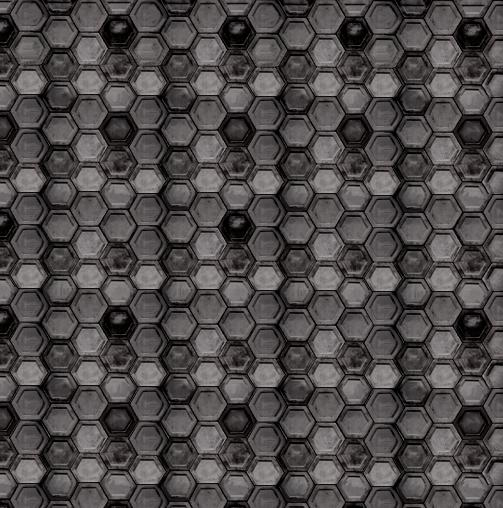
\includegraphics[width=0.2\textwidth]{Images/textures/airbase_radar_panels.jpg} &
\makecell[l]{Retrieved on the 8.12.2018 from \\ \linebreak https://opengameart.org/node/7254}
\end{tabular}
\end{centering}



\bibliographystyle{plain}
\bibliography{BachelorBooklet}

\listoffigures



\chapter*{Acknowledgments}
I like to thank Yannick Pawils for our daily insightful discussions and for his feedback which was a great guidance to me. \\
Also I like to thank my professor Thomas Bremer for the feedback and guidance he provided.\\
Furthermore I like to thank Susanne Brandhorst, Jules Pommier and Matthias Mayer.



\chapter*{Statement of Authorship}
I hereby declare that I am the sole author of this bachelor thesis and that I have not used any sources other than those listed in the bibliography- and resources section. I further declare that I have not submitted this thesis at any other institution in order to obtain a degree.
\begin{spacing}{5}
\null
\begin{spacing}{1}
\noindent
\dotfill \space \space \dotfill \\
(Place, Date) \hfill (Signature)\hfill \null
\end{spacing}
\end{spacing}



\newpage
\pagestyle{empty}
\centering
\vfill

\includegraphics[width=0.5\textwidth]{Images/logo_GD_black.jpg}
\vfill
\vspace*{-2cm}

\includegraphics[width=0.5\textwidth]{Images/logo_dehive.jpg}
\vfill

\includegraphics[width=0.5\textwidth]{Images/logo_htw.jpg}
\vfill



%\newpage
\blankpage
\blankpage
\blankpage

\begin{tikzpicture}[remember picture,overlay]
\node[inner sep=0pt] (background) at (current page.center) {
\includegraphics[width=\paperwidth]{Images/BackCover.png}};
\end{tikzpicture}

\finalcommand
\end{document}
